\documentclass[12pt,a4paper]{article}
\usepackage[top=1in, bottom=1in, left=1in, right=1in]{geometry}
\usepackage[utf8]{inputenc}

\usepackage{multicol}
\usepackage{hyperref}
\usepackage{newunicodechar}
\usepackage{graphicx}
\newunicodechar{😉}{
\includegraphics{figures/emoji_smile}}
\newunicodechar{💜}{
\includegraphics{figures/emoji_heart}}


\usepackage[intlimits]{amsmath}
\usepackage{amsmath}
\usepackage{amssymb}
\usepackage{amsthm}
\usepackage{latexsym}
\usepackage{graphicx}
% \usepackage[small]{caption2}
\usepackage{graphics}
% \usepackage{cite}

\usepackage[square,numbers,sort&compress]{natbib}

\newcommand{\Real}{\mathbb{R}}

\title{Character-level RNN Chatbot}
\author{Ivan Nazarov and Yermek Kapushev}
% \date{}

\begin{document}
\maketitle


\begin{section}{Introduction}
This project concerns development of a chatbot that can conduct natural conversation
similar to human ones.
The chatbot will be based on Recurrent Neural Network (RNN) and machine translation like architecture.

Long conversations are difficult to handle, so in this project we start from short-text conversations,
where the goal is to create a single response to a single query.
Then we try to incorporate some short chat history to keep track of what had been said.
\end{section}


\begin{section}{Data}
There were 2 data sets were used to train neural networks:
\begin{itemize}
    \item Cornell Movie Dialogues Corpus --- data set of dialogues from movies. The data set is split into dialogues, each dialogue can consist of several utterances. However, as they are dialogues from movies some of them don't sound very naturally.
    Here are some examples:\\

    \vspace{-1em}
    \footnotesize{
    $>$ Swear.\\
    $>$ What?\\
    $>$ Just say "I swear I won't kill anyone."\\
    }
    ---------

    \vspace{-1em}
    \footnotesize{
    $>$ "A History of the United States, Volume I." If you want to read a
    real history book, read Howard Zinn's "A People's History of
    the United States." That book will knock you on your ass.\\
    $>$ How about Noam Chomsky's "Manufacturing Consent?"\\
    $>$ You people baffle me. You spend all this money on beautiful,
    fancy books- and they're the wrong fuckin' books.\\
    $>$ You think so?\\
    $>$ Whatever blows your hair back.\\
    }

    \item \normalsize Twitter --- a data set of twits and responding twits. This one is more natural, and there can be a lot of slang, emojis and so on. Some examples:\\

    \vspace{-1em}
    \footnotesize{
    $>$ lol i texted that to my hubby when i saw him wink haha too funny
    he thought it was funny!\\
    $>$ not once, but twice! 😉\\
    }
    ---------

    \vspace{-1em}
    \footnotesize{
    $>$ in "shock" after fire wipes out country store this am.
    story tonight at 6pm after football on\\
    $>$ no way! we 💜 that place.\\
    }
\end{itemize}


Preprocessing was rather simple: character-level RNN is used in this project, so we just
leave alphanumerics, punctuation and the most frequent emojis.

\end{section}

\begin{section}{Base architecture}
Our base architecture is seq2seq model \cite{2015arXiv150605869V}.
It consists of two RNN: one RNN encodes input sequence (encoder) and one RNN decodes output
sequence (see Fig. \ref{fig:seq2seq_train} and \ref{fig:seq2seq_eval}).
Initially, we aimed at implementing adversarial training of sequence generator,
so in our implementation the output elements of decoder are generated using Gumbel-Softmax
sampling \cite{2016arXiv161104051K}, which is a continuous approximation of the categorical
distribution over characters. However, we then take just $\arg \max$, so there is no
difference with the original architecture. Adversarial training is left for future work.

We use character-level RNN for encoder and decoder. The following parameters were used:
\begin{itemize}
    \item number of layers in RNN --- $2$.
    \item RNN cell --- GRU.
    \item Number of hidden units in RNN cell --- $256$.
    \item Embedding size --- $32$.
\end{itemize}

\begin{figure}
    \centering
    % \hspace*{-7em}
    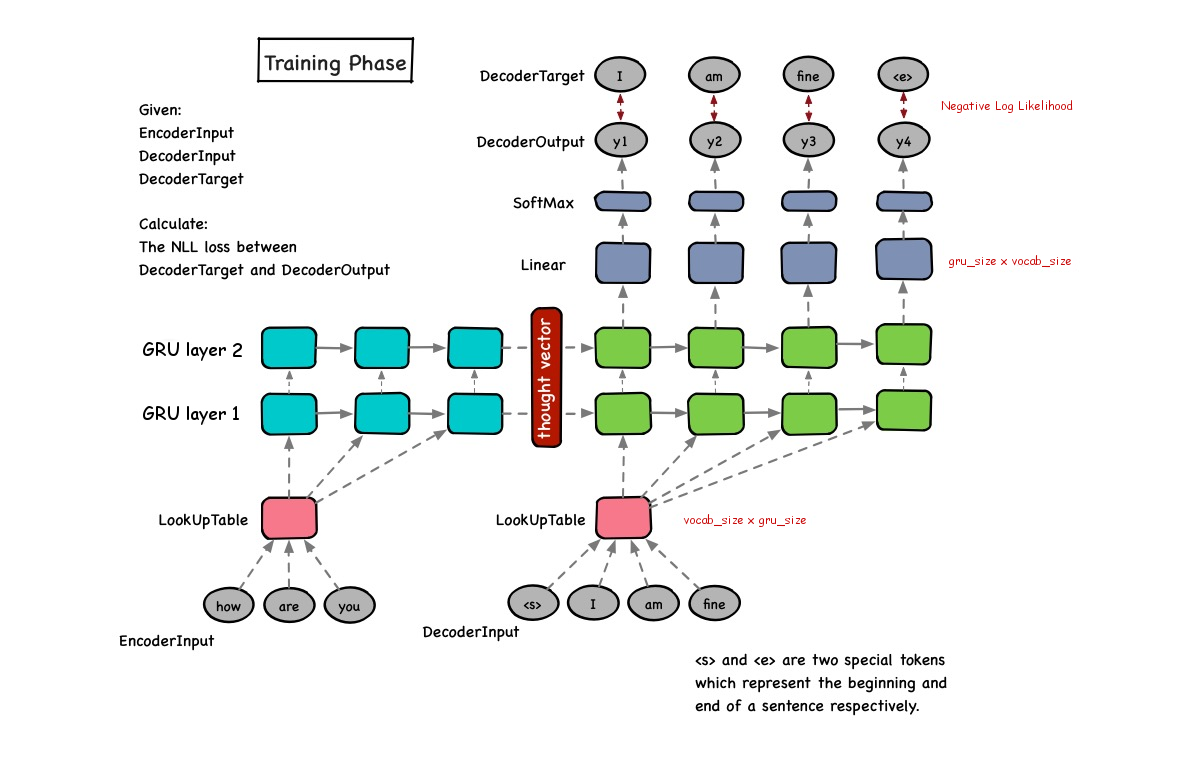
\includegraphics[width=0.8\textwidth]{figures/training.png}
    \caption[caption with fn]{Sequence to Sequence model architecture (training phase)\protect\footnotemark.}
    \label{fig:seq2seq_train}
\end{figure}

\footnotetext{\url{https://github.com/saltypaul/Seq2Seq-Chatbot}}

\begin{figure}
    \centering
    % \hspace*{-7em}
    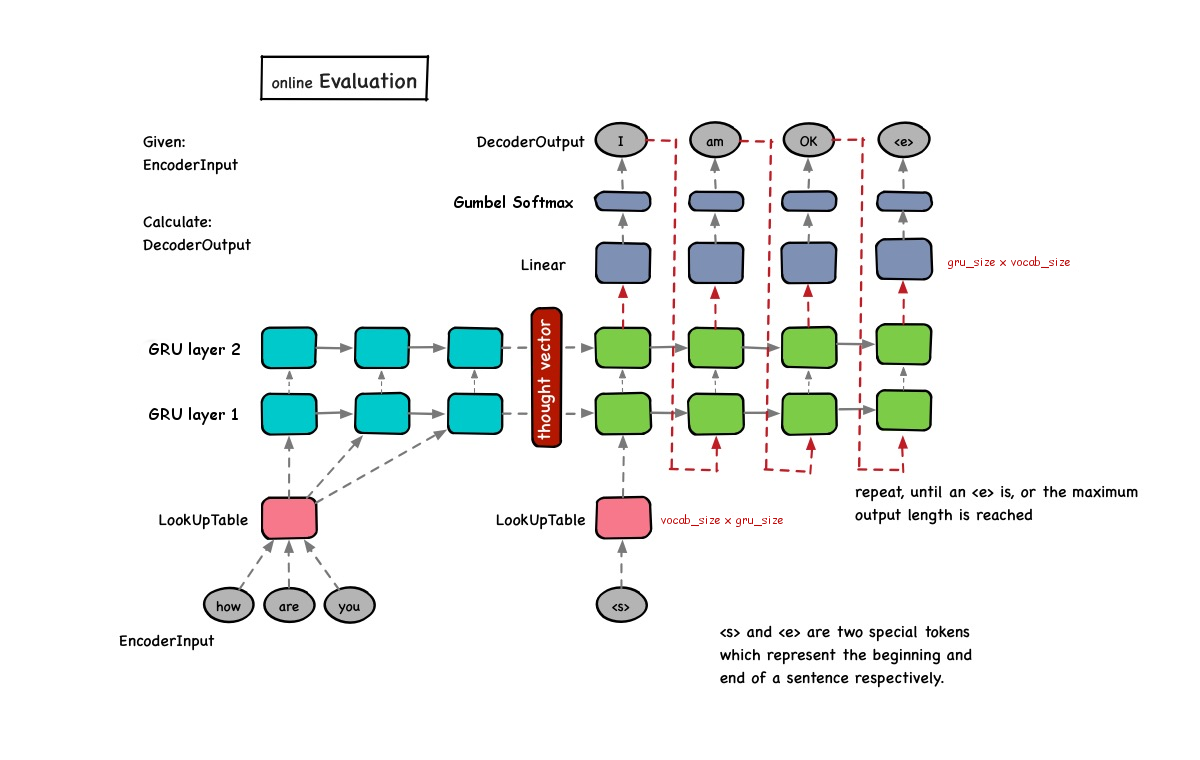
\includegraphics[width=0.8\textwidth]{figures/generation.png}
    \caption{Sequence to Sequence model architecture (evaluation phase)\protect\footnotemark.}
    \label{fig:seq2seq_eval}
\end{figure}


Here is an example of chat with bot:
{\footnotesize{
\begin{verbatim}
    Human   > Hey bot, tell something nice
    Machine < What?
    Human   > I don't know... A joke
    Machine < Larry, you've got to do something to do with. Without us...
    Human   > Hahaha. Let's pretend this is funny
    Machine < Okay.
    Human   > Do you think you are smart?
    Machine < I don't understand.
    Human   > You are stupid!
    Machine < I think I wouldn't let you marry anybody.
    Human   > Such a touchy bot..
    Machine < What are you talking about?
\end{verbatim}
}
}
\normalsize
As you can see, sometimes it kind of works, sometimes it doesn't work and generates inconsistent replies.

\footnotetext{\url{https://github.com/saltypaul/Seq2Seq-Chatbot}}
\end{section}


\begin{section}{Dialogue context}
In order to incorporate dialogue context to make bot to take into account some short chat history
the following architecture is used.
The decoder part remains the same.
Encoder part is depicted in figure \ref{fig:dialogue_context}.
It consists of 2 subnetworks.
The first one takes as input not one utterance, but several consequent utterances, i.e. 3 most recent
utterances: question, answer, question. It encodes each utterance into encoder's hidden state.
Then encoded utterances are passed to the second subnetwork as one input sequence.
As a result we obtain a hidden representation of a dialogue which is then passed to the decoder.

Here are two examples of the resulting model
\begin{multicols}{2}
\begin{itemize}
    \item Kind of working:
    \footnotesize{
    \begin{verbatim}
    Human   > What is the weather like today?
    Machine < You hate me.
    Human   > Yes, I do!
    Machine < You're right!
    Human   > I am always right, bot!
    Machine < Why?
    Human   > I AM YOUR FATHER!
    Machine < Yeah. Yeah.
    \end{verbatim}
    }
    \item \normalsize Not working
    \footnotesize{
    \begin{verbatim}
    Human   > Hi, bot
    Machine < What?
    Human   > How are you?
    Machine < What?
    Human   > What is the weather like today?
    Machine < Speaking of the school-
    Human   > You are not so smart as we expected!
    Machine < S
    \end{verbatim}
    }
\end{itemize}
\end{multicols}

\begin{figure}
    \centering
    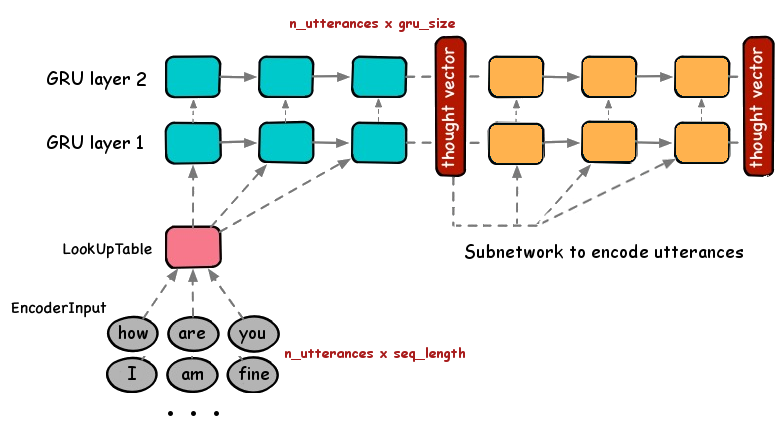
\includegraphics[width=0.6\textwidth]{figures/dialogue_context.png}
    \caption{Encoder with dialogue context.}
    \label{fig:dialogue_context}
\end{figure}
\end{section}

\section{RNN with attention model} % (fold)
\label{sec:rnn_with_attention_model}

With this architecture we tried to improve the quality of chatbot responses by
allowing it access to the full internal state of the encoder part, instead of
just the final hidden state as in fig.~\ref{fig:seq2seq_train}. To this end we
used the RNN with attention model described in \cite{2014arXiv14090473B}, which
gives the recurrent layer the ability to dynamically choose extra input from the
context sequence, see fig.~\ref{fig:attn_mech}. This enhanced RNN was used in
the decoder part of the network.

\begin{figure}[b]
    \centering
    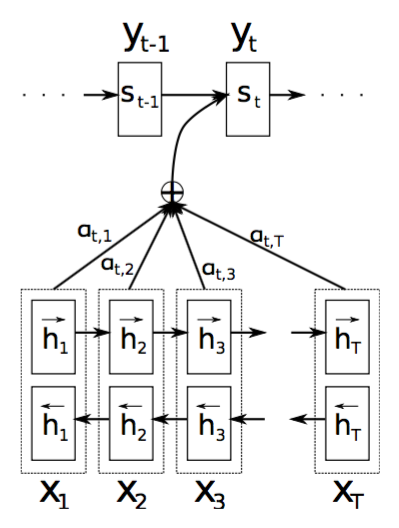
\includegraphics[width=0.3\textwidth]{figures/attn_mechanism.png}
    \caption{Attention mechanism (see \cite{2014arXiv14090473B} fig.~1).}
    \label{fig:attn_mech}
\end{figure}

Suppose $(z_t)_{t=1}^{T_z} \in\Real^{d}$ are the true inputs to a RNN layer
(GRU units), which the layer can observe sequentially. Let $(x_t)_{t=1}^{T_x}\in\Real^{m}$
be the sequence of contexts the layer has access to and which it can observe in
full. Furthermore let $(h_t)_{t=1}^{T_z}\in\mathbb{n}$ denote the hidden states
of the GRU units. Then the unit with attention mechanism has the similar dynamic
equations for its hidden states as the regular GRU unit, but with extra input
$\hat{x}_t$ derived from a context sequence:
\begin{align*}
    u_t &= \sigma(W_{uz} z_t + W_{uh} h_{t-1} + W_{ux} \hat{x}_t + b_u)
        \,, \tag{\text{UPDATE}} \\
    r_t &= \sigma(W_{rz} z_t + W_{rh} h_{t-1} + W_{rx} \hat{x}_t + b_r)
        \,, \tag{\text{RESET}}  \\
    \hat{h}_t &= \tanh\bigl(W_{hz} z_t + (W_{hh} h_{t-1})\odot r_t + W_{hx} \hat{x}_t + b_h\bigr)
        \,, \tag{\text{STATE}} \\
    h_t &= (1 - u_t)\odot h_{t-1} + u_t \odot \hat{h}_t
        \,,
\end{align*}
where the weights matrices are $W_{\cdot z}\in\Real^{n\times d}$,
$W_{\cdot x}\in\Real^{n\times m}$, $W_{\cdot h}\in\Real^{n\times n}$, and
$b_\cdot$ are the bias terms. The vector inputs $\hat{x}_t\in\Real^{m}$ are
determined in the following way:
\begin{align*}
    \hat{x}_t &= \sum_{s=1}^{T_x} \alpha_{ts} x_s
        \,,\,
    \alpha_{ts} = \frac{e^{w_{ts}}}{\sum_{k=1}^{T_x} e^{w_{tk}}}
        \,, \tag{\text{ATTN}}\\
    w_{ts} &= v' \tanh(W_{gh} h_{t-1} + W_{gx} x_s + b_w)
        \,,
\end{align*}
with $W_{gh}\in\Real^{q\times n}$, $W_{gx}\in\Real^{q\times m}$, $v\in\Real^q$ where
$q$ being the dimensionality of the attention module.

We tested the following architecture:
\begin{itemize}
    \item \textbf{Encoder}: bidirectional RNN consisting of GRU units with $256$ units;
    \item \textbf{Decoder}: $2$ forward layers of GRU, augmented with Attention model:
        \begin{itemize}
            \item the context sequence $x_i$ is the concatenation of the hidden
            states of the encoder's bi-di GRU units for input element $c_i$;
            \item the input sequence $z_t$ is the response character sequence,
            or the output of the layer below ($h^{(l-1)}_t$);
            \item the parameters: $m=512$, $n=256$, and $q=256$ for both layers;
        \end{itemize}
\end{itemize}
Here is a sample of the ``conversation'', which show that the trained chatbot gets
some idea of what is being asked: 
\footnotesize{
\begin{verbatim}
    Human   > You smart?
    Machine < Yes.
    Human   > really?
    Machine < Yes, son.
    Human   > are you sure?
    Machine < Of course.
    Human   > are you very very very very sure?
    Machine < Yes.
    Human   > Well, I think that you're dumb!
    Machine < I don't think so.
    Human   > Why don't you?
    Machine < I don't know that. Go to you. Yes, thank you.
              I've been sleeping. Why not?
    Human   > yeah, to some extent you were sleeping before I booted you.
    Machine < I wasn't doin' it.
    Human   > Okay, it seems as though you don't care about what I say to you, do you?
    Machine < Yes, I know.
    Human   > So you admit that you ignore the question part?
    Machine < Yes.
\end{verbatim}
}

% section rnn_with_attention_model (end)

\begin{section}{Stack-augmented RNN}
In this architecture we are trying to explicit memory via persistent stack, i.e. we
want our model to memorize states it sees important in the sequence and use it to
improve reply consistency. The architecture we have implemented is called Stack-Augmented
RNN \cite{2015arXiv150301007J}.

In this architecture both encoder and decoder share a common stack (see Fig. \ref{fig:stack}).
Each cell of RNN can write (push operation) and extract (pop operation) information
from the stack or do nothing (no-op operation).

Update rules for the cell hidden state and stack states are the following
\begin{align*}
h_t = & \sigma(U x_t + R h_{t - 1} + P s_{t-1}[\text{:k}]) \\
s_t[0] = & a_t[\texttt{PUSH}]\sigma(D h_t)
        + a_t[\texttt{POP}]s_{t-1}[1]
        + a_t[\texttt{NO-OP}]s_{t-1}[0] \\
s_t[i] = & a_t[\texttt{PUSH}]s_{t-1}[i-1]
        + a_t[\texttt{POP}]s_{t-1}[i+1]
        + a_t[\texttt{NO-OP}]s_{t-1}[i] \\
a_t = & \texttt{softmax}(A h_t)
\end{align*}
where $a_t[\cdot]$ is the probability of taking the corresponding action,
and $s_{t-1}[:k]$ is the vector of flattened (vec) top $k$ elements at the
top of the stack.

Here is an example of the result:
\footnotesize{
\begin{verbatim}
    Human   > So what are you doing?
    Machine < Maybe not only the time. I have to get
    Human   > What?
    Machine < It's my problem.
    Human   > But maybe I can help?
    Machine < You don't have to be?
    Human   > I don't understand
    Machine < What do you mean you get me to do to?
\end{verbatim}
}

\normalsize
The results are not satisfactory. The replies are inconsistent with the query. The
hypothesis is that we used character-level RNN, the network memorizes states related
to individual characters, which doesn't seem to have no much sense.

\begin{figure}
    \centering
    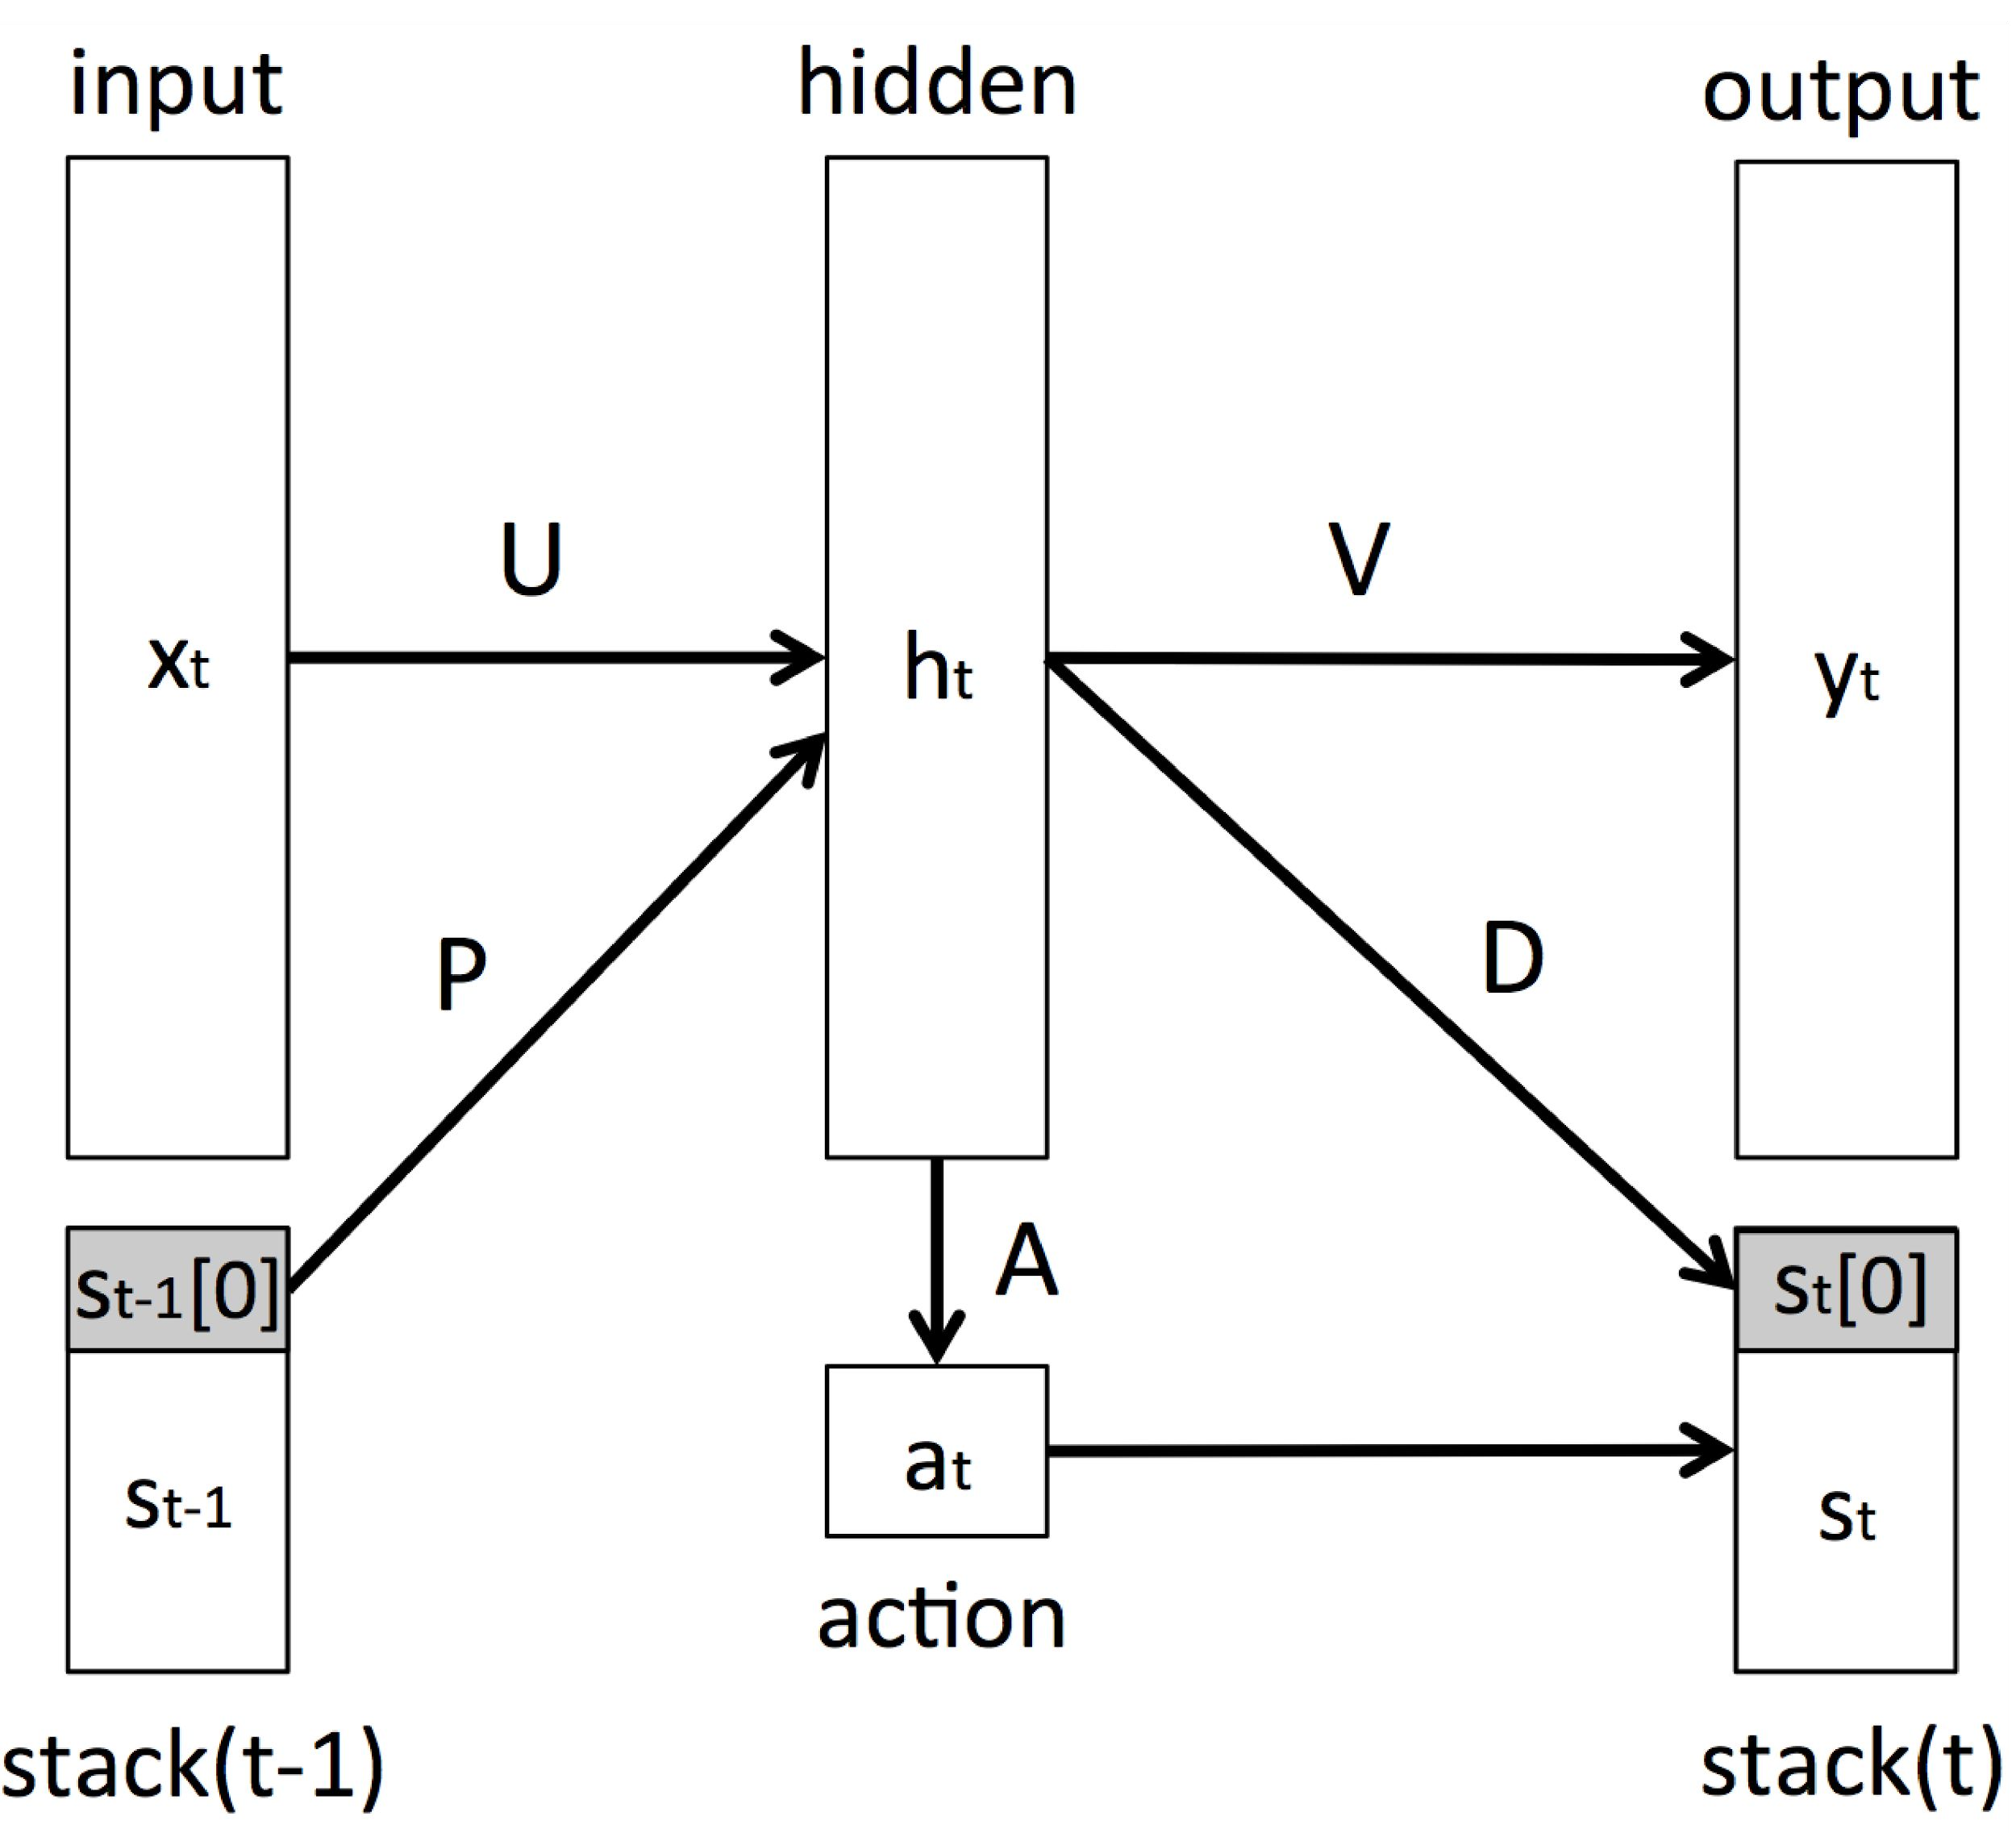
\includegraphics[width=0.3\textwidth]{figures/stack.png}
    \caption{Stack architecture (see \cite{2015arXiv150301007J} fig.~1).}
    \label{fig:stack}
\end{figure}


\end{section}

\begin{section}{Conclusions}
Our modest results show that simple 2 layered character-level RNN can generate basic
conversations, albeit with little coherency. We suspect that the root of the problem
is the lack of explicit persistent memory in the encoder-decoder pair, into
which both parts can tap for better representation extraction and sequence generation.

We have tried four seq-2-seq architectures: regular as in \cite{2015arXiv150605869V},
with explicit dialogue context, GRU RNN with attention mechanism over the encoder's
hidden state sequence, and stack augmented GRU RNN with shared stack. Unfortunately,
none of these approaches give satisfactory results: the chatbot does not exhibit
signs of understanding the queries in a manner, which is consistent with non-random
replies. Furthermore, neither stack, nor the explicit context dialogue seem to result
in thought persistence in the trained chat bot.

One possible reason for this is that all featured architectures use narrow recurrent
layers with $256-512$ units, while the typical width of recurrent layers in language
models is about $1000$ units. Another possible reason is the used dataset: the movie
dialogues can be excessively dramatic, provide too much exposition and be otherwise
unnatural in casual conversational situations like simple chat. Finally, despite
character-level RNNs capability to learn natural languages to high degree of realism,
still it is possible tha individual character is too a small semantic unit for both
the attention and memory mechanisms to benefit character level neural conversation
models.

Future work on this project might include:
\begin{itemize}
    \item use word-level embedding instead of character-level;
    \item attempt RL approach with explicit persistent state: end-to-end memory as
    in \cite{2015arXiv150308895S};
\end{itemize}

\end{section}

\begin{section}{Work distribution}

The code for the project is available at \url{https://github.com/ivannz/dl2017chatbot}.
\begin{itemize}
    \item \textbf{Ivan Nazarov:} initial research, most of the implementation,
    training the models, presenting the results;
    \item \textbf{Yermek Kapushev:} dataset collection, initial research, training
    the models, presenting the results, writing report.
\end{itemize}

\end{section}

% Citations
\nocite{*}
\bibliographystyle{plain}
\bibliography{references}

% \begin{thebibliography}{9}
% \bibitem{2015arXiv150605869V}
%     Vinyals, O., \& Le, Q. (2015).
%     A neural conversational model.
%     arXiv preprint arXiv:1506.05869.
% \bibitem{2014arXiv1409.0473B}
%     Joulin, A., \& Mikolov, T. (2015).
%     Inferring algorithmic patterns with stack-augmented recurrent nets.
%     \emph{In Advances in neural information processing systems} (pp. 190-198).
% \bibitem{2016arXiv161104051K}
%     Kusner, M. J., \& Hernández-Lobato, J. M. (2016).
%     GANS for Sequences of Discrete Elements with the Gumbel-softmax Distribution.
%     arXiv preprint arXiv:1611.04051.
% \end{thebibliography}

\end{document}
